\documentclass[aspectratio=169]{beamer}

\mode<presentation>
{
  \usetheme{default}
  \usecolortheme{default}
  \usefonttheme{default}
  \setbeamertemplate{navigation symbols}{}
  \setbeamertemplate{caption}[numbered]
  \setbeamertemplate{footline}[frame number]  % or "page number"
  \setbeamercolor{frametitle}{fg=white}
  \setbeamercolor{footline}{fg=black}
} 

\usepackage[english]{babel}
\usepackage[utf8x]{inputenc}
\usepackage{tikz}
\usepackage{courier}
\usepackage{array}
\usepackage{bold-extra}
\usepackage{minted}
\usepackage[thicklines]{cancel}

\xdefinecolor{dianablue}{rgb}{0.18,0.24,0.31}
\xdefinecolor{darkblue}{rgb}{0.1,0.1,0.7}
\xdefinecolor{darkgreen}{rgb}{0,0.5,0}
\xdefinecolor{darkgrey}{rgb}{0.35,0.35,0.35}
\xdefinecolor{darkorange}{rgb}{0.8,0.5,0}
\xdefinecolor{darkred}{rgb}{0.7,0,0}
\definecolor{darkgreen}{rgb}{0,0.6,0}
\definecolor{mauve}{rgb}{0.58,0,0.82}

\title[2018-02-05-cmsoffline-oamap]{Data Analysis R\&D}
\author{Jim Pivarski}
\institute{Princeton University -- DIANA-HEP}
\date{February 5, 2018}

\begin{document}

\logo{\pgfputat{\pgfxy(0.11, 7.4)}{\pgfbox[right,base]{\tikz{\filldraw[fill=dianablue, draw=none] (0 cm, 0 cm) rectangle (50 cm, 1 cm);}\mbox{\hspace{-8 cm}
\includegraphics[height=1 cm]{princeton-logo-long.png}
\includegraphics[height=1 cm]{diana-hep-logo-long.png}}}}}

\begin{frame}
  \titlepage
\end{frame}

\logo{\pgfputat{\pgfxy(0.11, 7.4)}{\pgfbox[right,base]{\tikz{\filldraw[fill=dianablue, draw=none] (0 cm, 0 cm) rectangle (50 cm, 1 cm);}\mbox{\hspace{-8 cm}
\includegraphics[height=1 cm]{princeton-logo.png}
\includegraphics[height=1 cm]{diana-hep-logo.png}}}}}

% Uncomment these lines for an automatically generated outline.
%\begin{frame}{Outline}
%  \tableofcontents
%\end{frame}

% START START START START START START START START START START START START START

\begin{frame}{Tools for data analysis}
\vspace{0.5 cm}
\begin{block}{\underline{Eventual goal}}
\vspace{0.15 cm}
{\bf Query-based analysis:} let physicists do their analysis by querying a central dataset instead of downloading and managing private skims. {\it Remove an expensive middleman!}
\end{block}

\vspace{0.5 cm}
\begin{block}{\underline{Existence proof}}
\begin{enumerate}
\item I've worked with such systems at several large companies as a statistical consultant, regularly querying terabytes in seconds.
\item Just to prepare this talk, I ran a query on Google BigQuery (2~TB in 30~sec).

Analysis-as-a-service is common in industry: this one is publicly accessible.
\end{enumerate}
\end{block}
\end{frame}

\begin{frame}{Google BigQuery}
\vspace{0.5 cm}
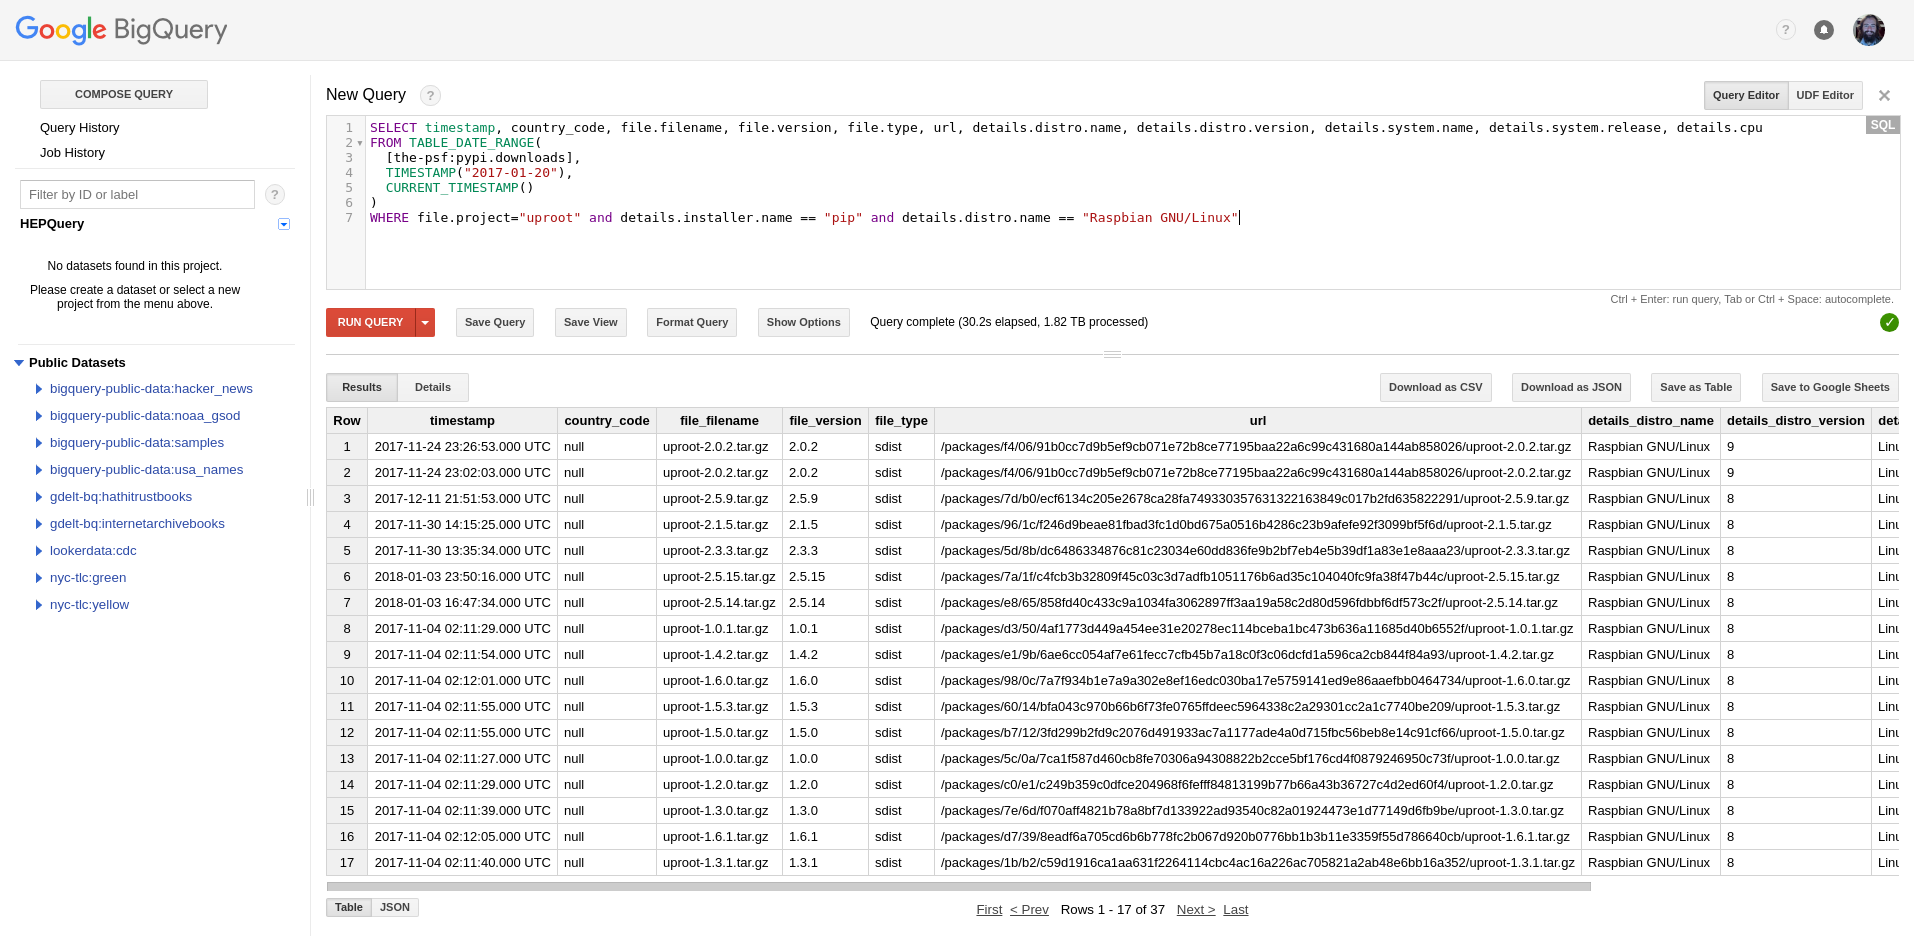
\includegraphics[width=\linewidth]{bigquery.png}
\end{frame}

\begin{frame}{These systems are not suited for HEP data, but they could be}
\vspace{0.25 cm}

\renewcommand{\arraystretch}{1.5}

\vspace{0.25 cm}\mbox{\hspace{-0.7 cm}
\begin{tabular}{p{0.26\linewidth} p{0.2\linewidth} p{0.21\linewidth} p{0.3\linewidth}}
& Google/Big Data & HEP & what I'm developing \\\hline
Source data format & \mbox{Parquet, ORC,} Avro, BSON, \ldots & ROOT & \mbox{{\bf uproot:} array-oriented} ROOT reader \\
Query language & SQL & Python or C++ & {\bf oamap:} columnar objects \\
Distributed storage & GFS/HDFS & {\it similar} (Ceph?) & {\it starting now} \\
Distributed processing & Dremel/Drill & \mbox{{\it similar} (Dask?} Zookeeper?) & {\it future} \\
User interface & \mbox{web dashboard,} \mbox{Google Sheets,} REST queries & TDataFrame, \mbox{PyROOT, Jupyter}, SWAN, Spark & {\bf Histogrammar:} \mbox{functional histogramming,} {\bf Femtocode} {\it (future)\ldots} \\
\end{tabular}}
\end{frame}

\begin{frame}{This talk: pieces that can be used on their own, right now}
\Large
\begin{description}
\item[{\bf uproot:}] pure-Python ROOT reader that directly copies columnar ROOT data into Numpy arrays.
\item[]
\item[{\bf oamap:}] object-array mapping (analogy to ORM) translating processes defined on virtual objects into operations on columnar arrays.
\end{description}
\end{frame}

\begin{frame}{Numpy is the reason an ML ecosystem developed in Python}
\vspace{0.5 cm}
\Large
Standardized way of wrapping low-level (fast) arrays in high-level (convenient) Python.

\vspace{0.75 cm}
Most scientific Python libraries are compiled code with Python interfaces, and Numpy is the standard way to move or share data between them.

\vspace{0.75 cm}
uproot provides this kind of access to ROOT.
\end{frame}

\begin{frame}[fragile]{Load one attribute for all events at a time}
\vspace{0.1 cm}
\small
\begin{minted}{python}
>>> import uproot
>>> t = uproot.open("tests/samples/Zmumu.root")["events"]
>>> t.keys()
\end{minted}
\begin{verbatim}
['Type', 'Run', 'Event', 'E1', 'px1', 'py1', 'pz1', 'pt1',
 'eta1', 'phi1', 'Q1', 'E2', 'px2', 'py2', 'pz2', 'pt2',
 'eta2', 'phi2', 'Q2', 'M']
\end{verbatim}
\begin{minted}{python}
>>> t["M"].array()
\end{minted}
\begin{verbatim}
array([ 82.46269156,  83.62620401,  83.30846467, ...,  95.96547966,
        96.49594381,  96.65672765])
\end{verbatim}
\begin{minted}{python}
>>> t.arrays(["px1", "py1", "pz1"])
\end{minted}
\begin{verbatim}
{'py1': array([ 17.433243, -16.5703623, -16.5703623, ..., 1.1994057,
 ...
\end{verbatim}
\begin{minted}{python}
>>> t.arrays()    # all of them!
\end{minted}
\begin{verbatim}
 ...
\end{verbatim}
\end{frame}

\begin{frame}[fragile]{Doing meaningful calculations with Numpy arrays}
\small
\begin{minted}{python}
>>> import uproot, numpy
>>> t = uproot.open("tests/samples/Zmumu.root")["events"]
>>> px, py, pz = t.arrays(["px1", "py1", "pz1"], outputtype=tuple)
>>> # compute pt for all events in the first pass
>>> pt = numpy.sqrt(px**2 + py**2)
>>> # compute eta for all events
>>> eta = numpy.arctanh(pz / numpy.sqrt(px**2 + py**2 + pz**2))
>>> # compute phi for all events
>>> phi = numpy.arctan2(py, px)
>>> print(pt, eta, phi)
\end{minted}
\begin{verbatim}
[ 44.7322 38.8311  38.8311  ...,  32.3997  32.3997 32.5076  ],
[-1.21769 -1.05139 -1.05139 ..., -1.57044 -1.57044 -1.57078 ],
[ 2.74126 -0.44087 -0.44087 ...,  0.03702  0.03702  0.036964]
\end{verbatim}

\normalsize
The loop over events is in (fast) compiled code, not (slow) Python for loops. When we iterate over big datasets, we iterate in batches:

\small
\begin{minted}{python}
uproot.iterate("files*.root", "events", ["px1"], entrystep=1000)
\end{minted}
\end{frame}

\begin{frame}[fragile]{Connector to an external package: Pandas}
\vspace{0.1 cm}
\small
\begin{minted}{bash}
$ pip install pandas --user
\end{minted}
\begin{minted}{python}
>>> df = t.pandas.df()   # all the same arguments as t.arrays()
>>> df
\end{minted}
\begin{verbatim}
              E1          E2      Event          M  Q1  Q2     Run  \
0      82.201866   60.621875   10507008  82.462692   1  -1  148031
1      62.344929   82.201866   10507008  83.626204  -1   1  148031
2      62.344929   81.582778   10507008  83.308465  -1   1  148031
3      60.621875   81.582778   10507008  82.149373  -1   1  148031
...
2302   1.199406 -26.398400  -74.532431 -153.847604   GT
2303   1.201350 -26.398400  -74.808372 -153.847604   GG

[2304 rows x 20 columns]
\end{verbatim}

\normalsize
Pandas is a Swiss army knife for {\it in-memory, tabular} data analysis. Linked to plotting tools, exploratory data analysis, and machine learning. The popular {\it Python for Data Analysis} book is basically a Pandas tutorial.
\end{frame}

\begin{frame}[fragile]{Data with non-uniform width (not scalar numbers)}
\vspace{0.1 cm}
\small
\begin{minted}{python}
>>> t = uproot.open("tests/samples/mc10events.root")["Events"]
>>> a = t.array("Muon.pt")    # such as std::vector<numbers>
>>> a                         # variable length for each event
\end{minted}
\begin{verbatim}
jaggedarray([[ 28.07074928],
             [],
             [ 5.52336693  5.4780116 4.13222885],
             ...
             [],
             [ 6.85138178],
             []])
\end{verbatim}
\begin{uncoverenv}<2->
\begin{onlyenv}<2>
\begin{minted}{python}
>>> for event in a:
...     for muon in event:
...         # conceptually, an array of different-length arrays
...
\end{minted}
\vspace{2 cm}
\end{onlyenv}
\begin{onlyenv}<1,3>
\begin{minted}{python}
>>> a.contents    # but efficiently stored as a contiguous block
\end{minted}
\begin{verbatim}
array([ 28.07074928,   5.52336693,   5.47801161,   4.13222885, ...
         5.06344414,   6.85138178], dtype=float32)
\end{verbatim}
\begin{minted}{python}
>>> a.stops       # with event boundaries in a separate array
\end{minted}
\begin{verbatim}
array([ 1,  1,  4,  7,  7,  8, 13, 13, 14, 14])
\end{verbatim}
\end{onlyenv}
\end{uncoverenv}
\end{frame}

\begin{frame}[fragile]{Not just TTrees; reads TStreamers and interprets several types}
\vspace{0.1 cm}
\small
\begin{minted}{python}
>>> import uproot
>>> f = uproot.open("mixed-data.root")
>>> f.allclasses()    # list object names and classes (recursively)
\end{minted}
\scriptsize
\begin{verbatim}
{'gaussian;1': <class 'uproot.rootio.TH1F'>, 'events;1': <class 'uproot.rootio.TTree>}
\end{verbatim}
\small
\begin{minted}{python}
>>> f["gaussian"].show()
\end{minted}
\scriptsize
\begin{verbatim}
                  0                                               2411
                  +--------------------------------------------------+
[-inf, -3)   0    |                                                  |
[-3, -2.4)   68   |*                                                 |
[-2.4, -1.8) 285  |******                                            |
[-1.8, -1.2) 755  |****************                                  |
[-1.2, -0.6) 1580 |**********************************                |
[-0.6, 0)    2296 |************************************************  |
[0, 0.6)     2286 |***********************************************   |
[0.6, 1.2)   1570 |*********************************                 |
[1.2, 1.8)   795  |****************                                  |
[1.8, 2.4)   289  |******                                            |
[2.4, 3)     76   |**                                                |
[3, inf]     0    |                                                  |
                  +--------------------------------------------------+
\end{verbatim}
\end{frame}

\begin{frame}{Other features}
\vspace{0.5 cm}
\Large
\begin{itemize}\setlength{\itemsep}{0.4 cm}
\item Explicit caching (user-provided {\large\tt dict} or {\large\tt dict}-like object)
\item Explicit parallel-processing \mbox{(user-provided {\large\tt ThreadPoolExecutor})\hspace{-1 cm}}
\item Optional non-blocking calls (useful when parallel-processing)
\item Lazy arrays (load on demand, aware of TBasket structure)
\item Numba integration: operations on Numpy arrays, JaggedArrays and TH1 can be compiled (more later)
\item Functional chains (like TDataFrame)
\end{itemize}
\end{frame}

\begin{frame}[fragile]{}
\vspace{0.5 cm}
\huge
\begin{center}
\begin{minipage}{0.8\linewidth}
\begin{verbatim}
pip install uproot --user
\end{verbatim}
\end{minipage}

\Large
\vspace{1 cm}
\href{https://github.com/scikit-hep/uproot}{\textcolor{blue}{https://github.com/scikit-hep/uproot}}

\vspace{0.5 cm}
\href{http://uproot.readthedocs.io}{\textcolor{blue}{http://uproot.readthedocs.io}}
\end{center}
\end{frame}

\begin{frame}{uproot download statistics (pip logs are in Google BigQuery)}
\vspace{0.25 cm}
\begin{columns}
\column{0.45\linewidth}
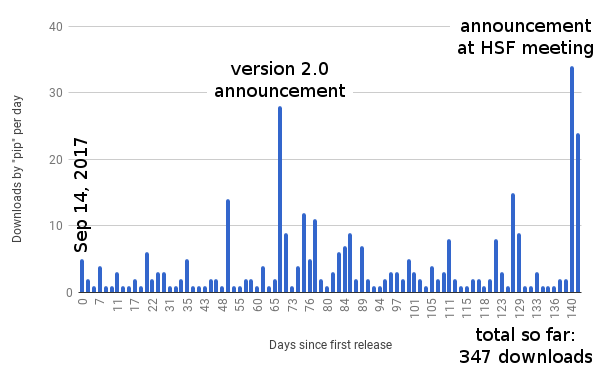
\includegraphics[width=\linewidth]{downloads-per-day.png}

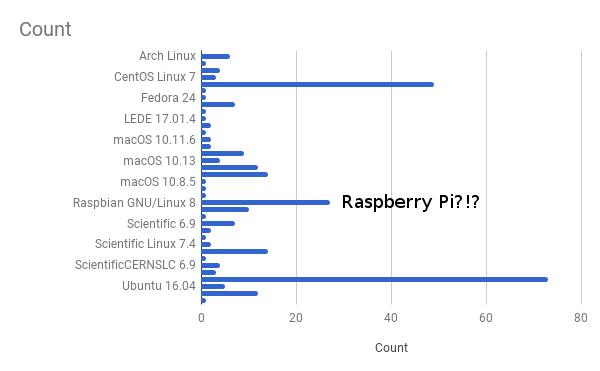
\includegraphics[width=\linewidth]{downloads-by-os.png}

\column{0.45\linewidth}
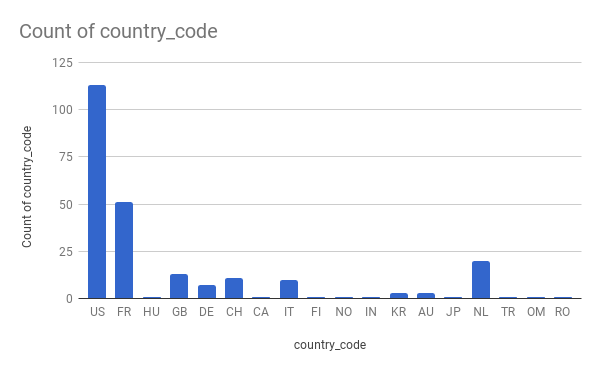
\includegraphics[width=\linewidth]{downloads-by-country.png}

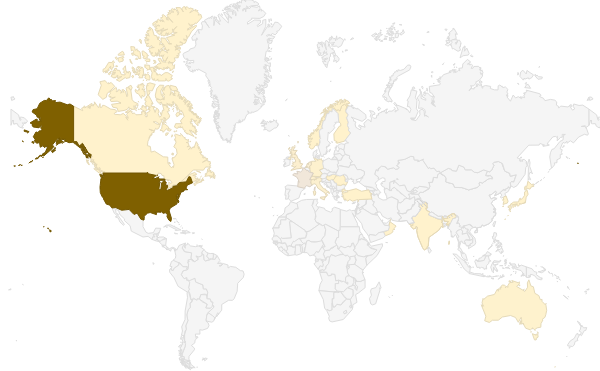
\includegraphics[width=\linewidth]{downloads-by-country-2.png}

\end{columns}
\end{frame}

\begin{frame}{Object-Array Mapping: generalizing JaggedArrays}
\vspace{0.5 cm}
JaggedArrays are only one data structure: list of lists of numbers.
\begin{itemize}
\item Implementation as an array of numbers with array of boundaries is much more efficient than thousands of tiny arrays randomly scattered in memory.
\item Sublists are ``views'' created on demand. (Not created at all in compiled code!)
\end{itemize}

\begin{uncoverenv}<2->
\vspace{0.25 cm}
\underline{\bf Generalize to a complete typesystem:}
\begin{description}
\item[primitives:] booleans, numbers, characters--- anything fixed-width;
\item[lists:] arbitrary length sequences of any single type;
\item[unions:] logical-or type (e.g.\ a Particle is an Electron or a Photon);
\item[records:] logical-and type: ``struct'' object that contains named, typed fields;
\item[tuples:] like a record, but typed fields are indexed, not named;
\item[pointers:] redirect to another collection to make trees, graphs, enumerations;
\item[extensions:] runtime interpretations of the above (e.g.\ list of chars as a ``string'').
\end{description}
\end{uncoverenv}
\end{frame}

\begin{frame}[fragile]{NASA Exoplanets example on website}
\vspace{0.1 cm}
\small
\begin{minted}{python}
>>> import oamap.source.parquet
>>> stars = oamap.source.parquet.open("planets*.parquet")
>>> stars
\end{minted}
\begin{verbatim}
[<Star at index 0>, <Star at index 1>, <Star at index 2>,
 <Star at index 3>, <Star at index 4>, ...]
\end{verbatim}
\begin{minted}{python}
>>> stars[0].ra, stars[0].dec
\end{minted}
\begin{verbatim}
(293.12738, 42.320103)
\end{verbatim}
\begin{minted}{python}
>>> stars[258].planets
\end{minted}
\begin{verbatim}
[<Planet at index 324>, <Planet at index 325>, <Planet at index 326>,
 <Planet at index 327>, <Planet at index 328>]
\end{verbatim}
\begin{minted}{python}
>>> [x.name for x in stars[258].planets]
\end{minted}
\begin{verbatim}
['HD 40307 b', 'HD 40307 c', 'HD 40307 d', 'HD 40307 f', 'HD 40307 g']
\end{verbatim}
\end{frame}

\begin{frame}[fragile]{Explore, scan with compiled code, then explore some more\ldots}
\vspace{0.1 cm}
\small
\begin{minted}{python}
>>> import numba             # compiles array-based Python code
>>> import oamap.compiler    # loads object-array compiler extensions
>>> @numba.njit              # decorator for compiling a function
>>> def orbital_period_ratio(stars):
...    out = []
...    for star in stars:
...       best_ratio = None
...       for one in star.planets:
...          for two in star.planets:
...             ratio = one.orbital_period.val / two.orbital_period.val
...             if best_ratio is None or ratio > best_ratio:
...                best_ratio = ratio
...       if best_ratio is not None and best_ratio > 200:
...          out.append(star)
...    return out
>>> extremes = orbital_period_ratio(stars)
>>> extremes
[<Star at index 284>, <Star at index 466>, <Star at index 469>, ...
\end{minted}
\end{frame}

\begin{frame}{oamap is an infrastructure component}
\vspace{0.5 cm}
\begin{itemize}\setlength{\itemsep}{0.25 cm}
\item TBranch data efficiently lifted from ROOT into arrays, efficiently scanned with oamap/numba-compiled functions.
\item Columns of data are {\it never} turned into objects.
\begin{itemize}
\item No need for schema evolution (no container classes).
\item ROOT-style selective and contiguous branch reading at all stages of the calculation: disk $\to$ memory and memory $\to$ CPU.
\item Alternate between object-oriented operations and vectorized (or GPU) operations.
\item Manipulate structure of dataset without copying data.
\item Different dataset versions can share the majority of their columns.
\end{itemize}
\item These techniques are common for SQL in databases, but new to full programming environments like Python objects.
\item There was nothing special about Python; this could be done for C++ as well.
\end{itemize}
\end{frame}

\begin{frame}[fragile]{}
\vspace{1 cm}
\huge
\begin{center}
\begin{minipage}{0.8\linewidth}
\begin{verbatim}pip install oamap --user
\end{verbatim}
\end{minipage}

\Large
\vspace{1 cm}
\href{https://github.com/diana-hep/oamap}{\textcolor{blue}{https://github.com/diana-hep/oamap}}
\end{center}

\normalsize
\vspace{1 cm}
(The demo examples use a Parquet file of NASA Exoplanets because I want it to be accessible to developers outside of HEP, to attract outside help.)
\end{frame}

\begin{frame}{Final slide: reminder of how these fit into a larger project}
\vspace{0.25 cm}

\renewcommand{\arraystretch}{1.5}

\vspace{0.25 cm}\mbox{\hspace{-0.7 cm}
\begin{tabular}{p{0.26\linewidth} p{0.2\linewidth} p{0.21\linewidth} p{0.3\linewidth}}
& Google/Big Data & HEP & what I'm developing \\\hline
Source data format & \mbox{Parquet, ORC,} Avro, BSON, \ldots & ROOT & \mbox{{\bf uproot:} array-oriented} ROOT reader \\
Query language & SQL & Python or C++ & {\bf oamap:} columnar objects \\
Distributed storage & GFS/HDFS & {\it similar} (Ceph?) & {\it starting now} \\
Distributed processing & Dremel/Drill & \mbox{{\it similar} (Dask?} Zookeeper?) & {\it future} \\
User interface & \mbox{web dashboard,} \mbox{Google Sheets,} REST queries & TDataFrame, \mbox{PyROOT, Jupyter}, SWAN, Spark & {\bf Histogrammar:} \mbox{functional histogramming,} {\bf Femtocode} {\it (future)\ldots} \\
\end{tabular}}
\end{frame}

\end{document}
